


\section{1. Moneyball}
\subsection{1.1}

{\it Visually explore the data. Plot the distribution of each feature (e.g. histograms), as well as the target. Visualize the dependency of the target on each feature (use a 2d scatter plot). Is there anything that stands out? Is there something that you think might require special treatment?
- Feel free to create additional plots that help you understand the data
- Only visualize the data, you don't need to change it (yet)} \\

The first column of figures shows the histograms of each column of the data in X. 
The second column shows the relationship between y and x. 

*Is there anything that stands out? Is there something that you think might require special treatment?*

The dataset containts missing values in column 9,10, 12 and 13 so the data set must first be pre-processed to visualize it. In order the scatterplot and histogram for the relevant features the NaN value were removed.
Beside the NaN the data the figures that do not show a clear distrubution are: 1, 8, 10 and 11, so these features may need further investigation as well. The relevant plots are visible in figure \ref{fig:scatter_hist}.\\

\begin{figure}

\centering    
\subfigure{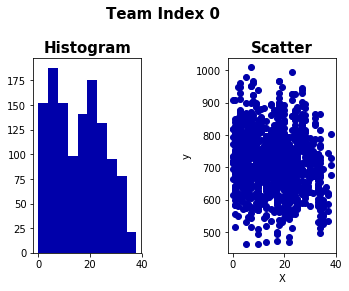
\includegraphics[width=40mm]{./Figures_1/output_5_141}}
\subfigure{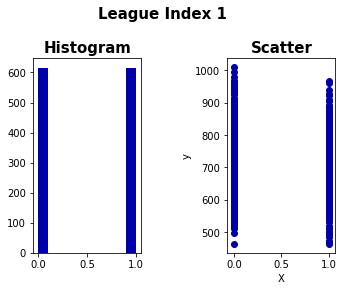
\includegraphics[width=40mm]{./Figures_1/output_5_142}}
\subfigure{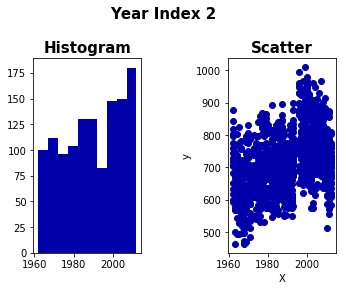
\includegraphics[width=40mm]{./Figures_1/output_5_143}}

\subfigure{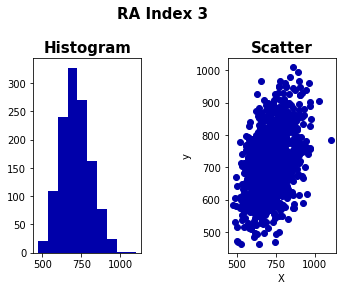
\includegraphics[width=40mm]{./Figures_1/output_5_144}}
\subfigure{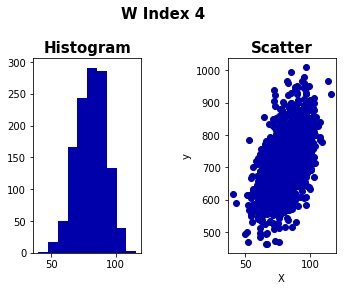
\includegraphics[width=40mm]{./Figures_1/output_5_145}}
\subfigure{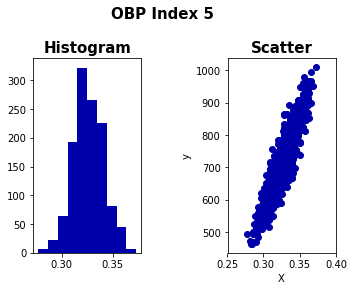
\includegraphics[width=40mm]{./Figures_1/output_5_146}}

\subfigure{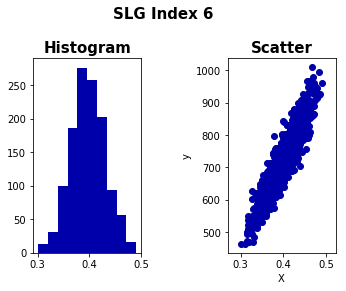
\includegraphics[width=40mm]{./Figures_1/output_5_147}}
\subfigure{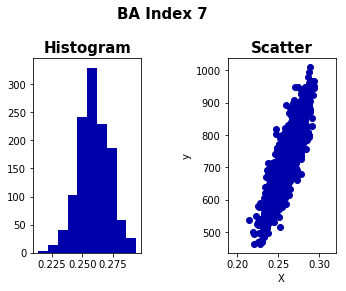
\includegraphics[width=40mm]{./Figures_1/output_5_148}}
\subfigure{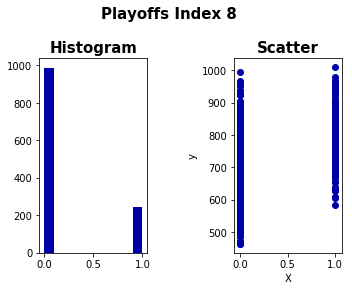
\includegraphics[width=40mm]{./Figures_1/output_5_149}}

\subfigure{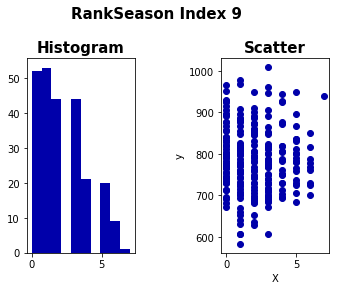
\includegraphics[width=40mm]{./Figures_1/output_5_150}}
\subfigure{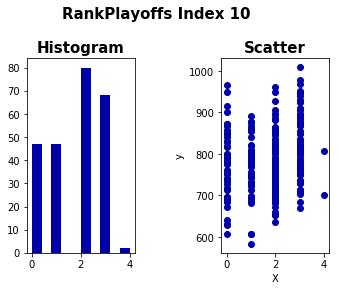
\includegraphics[width=40mm]{./Figures_1/output_5_151}}
\subfigure{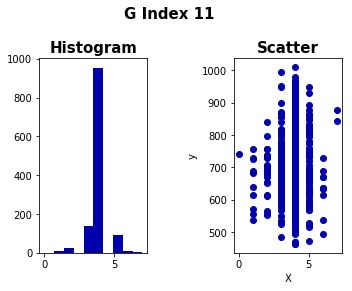
\includegraphics[width=40mm]{./Figures_1/output_5_152}}

\subfigure{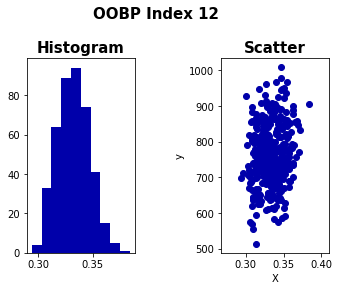
\includegraphics[width=40mm]{./Figures_1/output_5_153}}
\subfigure{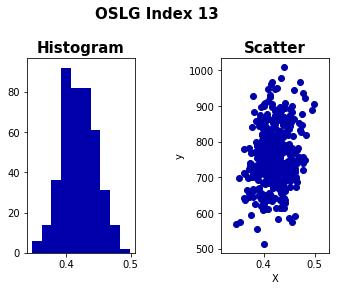
\includegraphics[width=40mm]{./Figures_1/output_5_154}}

\caption{Histograms and scatter plots of Moneyball features}
\label{fig:scatter_hist} %label altijd na caption..

\end{figure}

\subsection{1.2}
{\it Compare all linear regression algorithms that we covered in class (Linear Regression, Ridge, Lasso and ElasticNet), as well as kNN. Evaluate using cross-validation and the $R^2$ score, with the default parameters. Does scaling the data with StandardScaler help? Provide a concise but meaningful interpretation of the results.
- Preprocess the data as needed (e.g. are there nominal features that are not ordinal?). If you don't know how to proceed, remove the feature and continue.}\\

All features which have missing data were removed from the featureset before any further analysis. This means 4 features are removed completely and 10 features are considered for model generation. We chose to remove the data instead of filling in missing values because we were not sure which strategy to use for filling the blanks, and we assumed that using 10 out of the 14 features would still be enough to obtain sufficiently good models.

Without scaling, LinearRegression returns the best score at 0.92 and an r2 of 0.95. The other regression algorithms return worse, but still acceptable scores, with one exception: KNN yields a score of 0.00 and an r2 score of only 0.2. Most likely there is an error in how the KNN algorithm is used here, but we were unable to pinpoint the issue.

Using StandardScaler has no effect on the LinearRegression scores, but all other algorithms have significantly higher scores compared to their counterparts where scaling was not used. Ridge now matches the scores of LinearRegression, and Lasso comes close as well losing by 0.01 point in the r2 score. ElasticNet scores are also improved, but the scores are not as high as the other three algorithms. The KNN score improves sleightly but is still a lot lower then is to be expected. \\

A table containing all scores is visible in Table \ref{table:score_table}

\begin{table}[]
\centering
\caption{scoring data for several linear regression algorithms}
\label{table:score_table}
\begin{tabular}{lllll}
                  &       &      &                       &                    \\
                  & score & r2   & score\_StandardScaler & r2\_StandardScaler \\
Linear Regression & 0.92  & 0.95 & 0.92                  & 0.95               \\
Ridge             & 0.84  & 0.89 & 0.92                  & 0.95               \\
Lasso             & 0.80  & 0.86 & 0.92                  & 0.94               \\
KNN               & 0.00  & 0.20 & 0.01                  & 0.63               \\
ElasticNet        & 0.80  & 0.86 & 0.87                  & 0.90              
\end{tabular}
\end{table}


\subsection{1.3}
{\it Do a default, shuffled train-test split and optimize the linear models for the degree of regularization ($alpha$) and choice of penalty (L1/L2). For Ridge and  Lasso, plot a curve showing the effect of the training and test set performance ($R^2$) while increasing the degree of regularization for different penalties. For ElasticNet, plot a heatmap $alpha \times l1\_ratio \rightarrow R^2$ using test set performance.
Report the optimal performance. Again, provide a concise but meaningful interpretation. What does the regularization do? Can you get better results?
- Think about how you get the L1/L2 loss. This is not a hyperparameter in regression.
- We've seen how to generate such heatmaps in Lecture 3.} \\

To optimize alpha, a CVGridSearch was used. For Ridge ans Lasso, a logscale containing 100 samples from [0.001-100] were used as alpha parameter. For Ridge regression, alpha=0.001 returns the highest score, while for Lasso regression alpha=0.004 yielded the maximum score. Ridge regression performs L2 regularization, while Lasso regression performs L1 regularization, where alpha influences the L2/L1 penalty respectively. It is interesting to observe that for low values of alpha, Ridge and Lasso perform almost identically, as can be oberved in figure \ref{fig:ridgelasso}. It is interesting to note that the Lasso curve closely resembles a Tikhonov regularization L curve. \\

\begin{figure}
\centering    
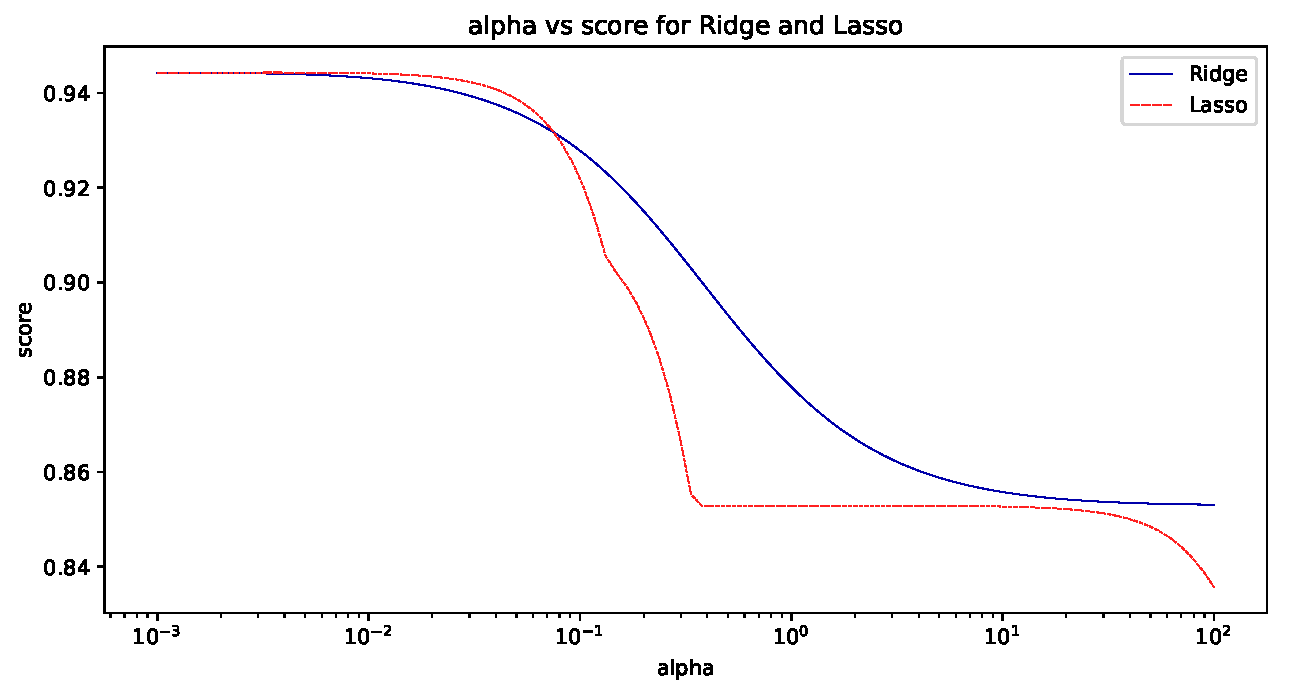
\includegraphics[width=120mm]{./Figures_1/ridgelasso}
\caption{score vs increasing regularization for Ridge and Lasso}
\label{fig:ridgelasso} %label altijd na caption..
\end{figure}

For ElasticNet 11 samples for the r1 ratio from [0-1]and 11 samples from[0.001-100] were used in the GridSearch. The highest scores are obtained with alpha=0.001, the lowest tested value for alpha, and an L1 ratio of 1. This is also clear from the heatmap in figure \ref{fig:elasticnet}. 
For KNN and LinearRegression no alpha hyperparameter exists, so these were not optimised.

\begin{figure}
\centering    
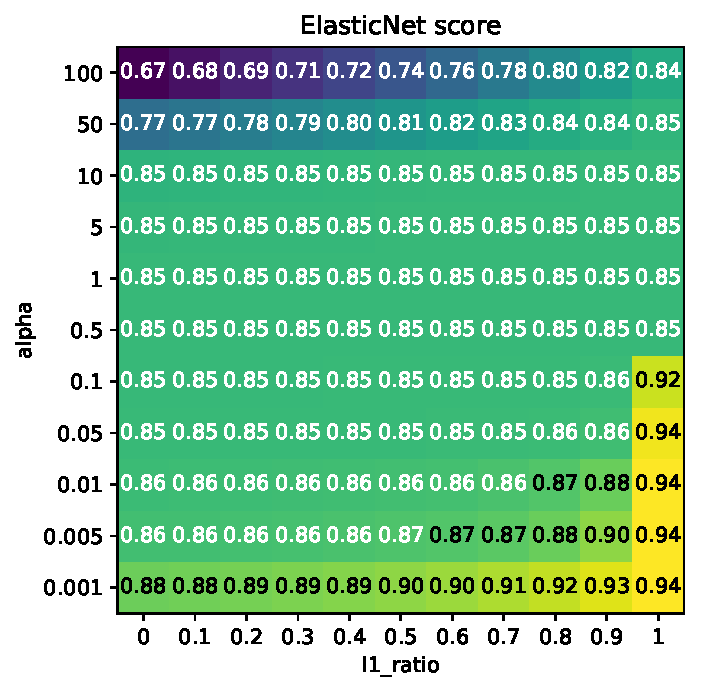
\includegraphics[width=100mm]{./Figures_1/elasticnet}
\caption{Histograms and scatter plots of Moneyball features}
\label{fig:elasticnet} %label altijd na caption..
\end{figure}

Higher scores might be obtained by trying a wider range of alpha values or using more samples per GridSearch. As seen in assignment 1.2, using a scaler may also lead to higher scores. A third option would be to use a RandomGridSearch which can try more values for alpha than the discrete steps used in a normal GridSearch. \\






\subsection{1.4}
{\it Visualize the coefficients of the optimized models. Do they agree on which features are
important? Compare the results with the feature importances returned by a RandomForest. Does it agree with the linear models? What would look for when scouting for a baseball player?}\\

LR, Ridge, Lasso and EN all seem to agree that the features with index 5 (OBP) is most important, followed closely by feature 6 (SLG). All other features have coefficients at least two orders of magnitude lower, so they hardly make a difference. Feature 5 (OBP) is On-Base Percentage, and feature 6 (SLG) is Slugging Percentage. However, the RandomForest paints a different picture entirely. While SLG and OBP are also relatively important according to the RandomForest, the Team, Year, BA, RA and W features get about the same importance scores. For all data, refer to table \ref{table:coefficients} and table \ref{table:rf}.

So, it seems deciding on important features to look for in Baseball players is not so clear cut. The linear models and RandomForest do agree on some features that are of lesser importance: League, Playoffs and G are features a scout does not need to pay attention to. \\

\begin{table}[]
\centering
\caption{Linear Regression coëfficients}
\label{table:coefficients}
\begin{tabular}{lllllllllll}
      & 0    & 1     & 2     & 3    & 4    & 5       & 6       & 7       & 8    & 11   \\
LR    & 0.07 & -4.56 & -0.33 & 0.27 & 2.61 & 2053.28 & 1203.09 & -119.03 & 1.43 & 4.08 \\
Ridge & 0.07 & -4.54 & -0.33 & 0.28 & 2.65 & 1997.63 & 1195.57 & -79.81  & 1.46 & 4.02 \\
Lasso & 0.07 & -4.49 & -0.32 & 0.28 & 2.74 & 1912.05 & 1172.60 & -0.00   & 1.47 & 3.91 \\
EN    & 0.07 & -4.54 & -0.33 & 0.27 & 2.64 & 2013.22 & 1193.86 & -74.72  & 1.45 & 4.05
\end{tabular}
\end{table}

\begin{table}[]
\centering
\caption{Random Forest feature importances}
\label{table:rf}
\begin{tabular}{lllllllllll}
   & 0      & 1      & 2      & 3      & 4      & 5      & 6      & 7      & 8      & 11     \\
RF & 0.1226 & 0.0311 & 0.1237 & 0.1398 & 0.1272 & 0.1213 & 0.1455 & 0.1312 & 0.0144 & 0.0433
\end{tabular}
\end{table}

